\documentclass[twoside,11pt]{article}
% Used for PODs
\def\C++{{\rm C\kern-.05em\raise.3ex\hbox{\footnotesize ++}}}
\def\underscore{\leavevmode\kern.04em\vbox{\hrule width 0.4em height 0.3pt}}
\setlength{\parindent}{0pt}

% +
%  Name:
%     sunxxx.tex

%  Purpose:
%     SUN documentation for ORAC-DR integral field unit (SUN/xxx)

%  Authors:
%    Stephen Todd (University of Edinburgh)

%  Copyright:
%     Copyright (C) 2002 Particle Physics and Astronomy
%     Research Council. All Rights Reserved.

%  History:
%     $Log$
%     Revision 1.1  2003/03/25 15:08:34  stodd
%     First version
%
%
%     Revision 1.0  March 2003
%     - First version

% -


% ? Specify used packages
\usepackage{graphicx}        %  Use this one for final production.
% \usepackage[draft]{graphicx} %  Use this one for drafting.
% ? End of specify used packages

\pagestyle{myheadings}

% -----------------------------------------------------------------------------
% ? Document identification
% Fixed part
\newcommand{\stardoccategory}  {Starlink User Note}
\newcommand{\stardocinitials}  {SUN}
\newcommand{\stardocsource}    {sun\stardocnumber}
\newcommand{\stardoccopyright} {Copyright \copyright\ 2003 Particle Physics and Astronomy Research Council}

% Variable part - replace [xxx] as appropriate.
\newcommand{\stardocnumber}    {246.1}
\newcommand{\stardocauthors}   {Stephen Todd \\
                                Edinburgh University}
\newcommand{\stardocdate}      {February 2003}
\newcommand{\stardoctitle}     {ORAC-DR -- integral field spectroscopy
  data reduction}
\newcommand{\stardocversion}   {0.4}
\newcommand{\stardocmanual}    {User Guide}
\newcommand{\stardocabstract}  {ORAC-DR is a
general-purpose automatic data-reduction pipeline environment.  This
document describes its use to reduce integral field unit (IFU) data
collected at the United Kingdom Infrared Telescope (UKIRT) with the
UIST instrument. }
% ? End of document identification
% -----------------------------------------------------------------------------

% +
%  Name:
%     sun.tex
%
%  Purpose:
%     Template for Starlink User Note (SUN) documents.
%     Refer to SUN/199
%
%  Authors:
%     AJC: A.J.Chipperfield (Starlink, RAL)
%     BLY: M.J.Bly (Starlink, RAL)
%     PWD: Peter W. Draper (Starlink, Durham University)
%
%  History:
%     17-JAN-1996 (AJC):
%        Original with hypertext macros, based on MDL plain originals.
%     16-JUN-1997 (BLY):
%        Adapted for LaTeX2e.
%        Added picture commands.
%     13-AUG-1998 (PWD):
%        Converted for use with LaTeX2HTML version 98.2 and
%        Star2HTML version 1.3.
%      1-FEB-2000 (AJC):
%        Add Copyright statement in LaTeX
%     {Add further history here}
%
% -

\newcommand{\stardocname}{\stardocinitials /\stardocnumber}
\markboth{\stardocname}{\stardocname}
\setlength{\textwidth}{160mm}
\setlength{\textheight}{230mm}
\setlength{\topmargin}{-2mm}
\setlength{\oddsidemargin}{0mm}
\setlength{\evensidemargin}{0mm}
\setlength{\parindent}{0mm}
\setlength{\parskip}{\medskipamount}
\setlength{\unitlength}{1mm}

% -----------------------------------------------------------------------------
%  Hypertext definitions.
%  ======================
%  These are used by the LaTeX2HTML translator in conjunction with star2html.

%  Comment.sty: version 2.0, 19 June 1992
%  Selectively in/exclude pieces of text.
%
%  Author
%    Victor Eijkhout                                      <eijkhout@cs.utk.edu>
%    Department of Computer Science
%    University Tennessee at Knoxville
%    104 Ayres Hall
%    Knoxville, TN 37996
%    USA

%  Do not remove the %begin{latexonly} and %end{latexonly} lines (used by 
%  LaTeX2HTML to signify text it shouldn't process).
%begin{latexonly}
\makeatletter
\def\makeinnocent#1{\catcode`#1=12 }
\def\csarg#1#2{\expandafter#1\csname#2\endcsname}

\def\ThrowAwayComment#1{\begingroup
    \def\CurrentComment{#1}%
    \let\do\makeinnocent \dospecials
    \makeinnocent\^^L% and whatever other special cases
    \endlinechar`\^^M \catcode`\^^M=12 \xComment}
{\catcode`\^^M=12 \endlinechar=-1 %
 \gdef\xComment#1^^M{\def\test{#1}
      \csarg\ifx{PlainEnd\CurrentComment Test}\test
          \let\html@next\endgroup
      \else \csarg\ifx{LaLaEnd\CurrentComment Test}\test
            \edef\html@next{\endgroup\noexpand\end{\CurrentComment}}
      \else \let\html@next\xComment
      \fi \fi \html@next}
}
\makeatother

\def\includecomment
 #1{\expandafter\def\csname#1\endcsname{}%
    \expandafter\def\csname end#1\endcsname{}}
\def\excludecomment
 #1{\expandafter\def\csname#1\endcsname{\ThrowAwayComment{#1}}%
    {\escapechar=-1\relax
     \csarg\xdef{PlainEnd#1Test}{\string\\end#1}%
     \csarg\xdef{LaLaEnd#1Test}{\string\\end\string\{#1\string\}}%
    }}

%  Define environments that ignore their contents.
\excludecomment{comment}
\excludecomment{rawhtml}
\excludecomment{htmlonly}

%  Hypertext commands etc. This is a condensed version of the html.sty
%  file supplied with LaTeX2HTML by: Nikos Drakos <nikos@cbl.leeds.ac.uk> &
%  Jelle van Zeijl <jvzeijl@isou17.estec.esa.nl>. The LaTeX2HTML documentation
%  should be consulted about all commands (and the environments defined above)
%  except \xref and \xlabel which are Starlink specific.

\newcommand{\htmladdnormallinkfoot}[2]{#1\footnote{#2}}
\newcommand{\htmladdnormallink}[2]{#1}
\newcommand{\htmladdimg}[1]{}
\newcommand{\hyperref}[4]{#2\ref{#4}#3}
\newcommand{\htmlref}[2]{#1}
\newcommand{\htmlimage}[1]{}
\newcommand{\htmladdtonavigation}[1]{}

\newenvironment{latexonly}{}{}
\newcommand{\latex}[1]{#1}
\newcommand{\html}[1]{}
\newcommand{\latexhtml}[2]{#1}
\newcommand{\HTMLcode}[2][]{}

%  Starlink cross-references and labels.
\newcommand{\xref}[3]{#1}
\newcommand{\xlabel}[1]{}

%  LaTeX2HTML symbol.
\newcommand{\latextohtml}{\LaTeX2\texttt{HTML}}

%  Define command to re-centre underscore for Latex and leave as normal
%  for HTML (severe problems with \_ in tabbing environments and \_\_
%  generally otherwise).
\renewcommand{\_}{\texttt{\symbol{95}}}

% -----------------------------------------------------------------------------
%  Debugging.
%  =========
%  Remove % on the following to debug links in the HTML version using Latex.

% \newcommand{\hotlink}[2]{\fbox{\begin{tabular}[t]{@{}c@{}}#1\\\hline{\footnotesize #2}\end{tabular}}}
% \renewcommand{\htmladdnormallinkfoot}[2]{\hotlink{#1}{#2}}
% \renewcommand{\htmladdnormallink}[2]{\hotlink{#1}{#2}}
% \renewcommand{\hyperref}[4]{\hotlink{#1}{\S\ref{#4}}}
% \renewcommand{\htmlref}[2]{\hotlink{#1}{\S\ref{#2}}}
% \renewcommand{\xref}[3]{\hotlink{#1}{#2 -- #3}}
%end{latexonly}
% -----------------------------------------------------------------------------
% ? Document specific \newcommand or \newenvironment commands.

\newcommand{\CCDPACK}{\xref{{\sc{Ccdpack}}}{sun139}{}}
\newcommand{\GAIA}{\xref{{\sc{Gaia}}}{sun214}{}}
\newcommand{\FIGARO}{\xref{{\sc{Figaro}}}{sun86}{}}
\newcommand{\KAPPA}{\xref{{\sc{Kappa}}}{sun95}{}}
\newcommand{\ORACDR}{{\footnotesize ORAC-DR}}


% ? End of document specific commands
% -----------------------------------------------------------------------------
%  Title Page.
%  ===========
\renewcommand{\thepage}{\roman{page}}
\begin{document}
\setcounter{secnumdepth}{5}
\thispagestyle{empty}

%  Latex document header.
%  ======================
\begin{latexonly}
   CCLRC / \textsc{Rutherford Appleton Laboratory} \hfill \textbf{\stardocname}\\
   {\large Particle Physics \& Astronomy Research Council}\\
   {\large Starlink Project\\ }
   {\large \stardoccategory\ \stardocnumber}
   \begin{flushright}
   \stardocauthors\\
   \stardocdate
   \end{flushright}
   \vspace{-4mm}
   \rule{\textwidth}{0.5mm}
   \vspace{5mm}
   \begin{center}
   {\Huge\textbf{\stardoctitle \\ [2.5ex]}}
   {\LARGE\textbf{\stardocversion \\ [4ex]}}
   {\Huge\textbf{\stardocmanual}}
   \end{center}
   \vspace{5mm}

% ? Add picture here if required for the LaTeX version.
%   e.g. \includegraphics[scale=0.3]{filename.ps}
\begin{center}

\includegraphics[width=1.0in]{orac_logo.eps}
\end{center}
% ? End of picture

% ? Heading for abstract if used.
   \vspace{10mm}
   \begin{center}
      {\Large\textbf{Abstract}}
   \end{center}
% ? End of heading for abstract.
\end{latexonly}

%  HTML documentation header.
%  ==========================
\begin{htmlonly}
   \xlabel{}
   \begin{rawhtml} <H1> \end{rawhtml}
      \stardoctitle\\
      \stardocversion\\
      \stardocmanual
   \begin{rawhtml} </H1> <HR> \end{rawhtml}

% ? Add picture here if required for the hypertext version.
%   e.g. \includegraphics[scale=0.7]{filename.ps}

\includegraphics[width=1.0in]{orac_logo.eps}
% ? End of picture

   \begin{rawhtml} <P> <I> \end{rawhtml}
   \stardoccategory\ \stardocnumber \\
   \stardocauthors \\
   \stardocdate
   \begin{rawhtml} </I> </P> <H3> \end{rawhtml}
      \htmladdnormallink{CCLRC / Rutherford Appleton Laboratory}
                        {http://www.cclrc.ac.uk} \\
      \htmladdnormallink{Particle Physics \& Astronomy Research Council}
                        {http://www.pparc.ac.uk} \\
   \begin{rawhtml} </H3> <H2> \end{rawhtml}
      \htmladdnormallink{Starlink Project}{http://www.starlink.rl.ac.uk/}
   \begin{rawhtml} </H2> \end{rawhtml}
   \htmladdnormallink{\htmladdimg{source.gif} Retrieve hardcopy}
      {http://www.starlink.rl.ac.uk/cgi-bin/hcserver?\stardocsource}\\

%  HTML document table of contents. 
%  ================================
%  Add table of contents header and a navigation button to return to this 
%  point in the document (this should always go before the abstract \section). 
  \label{stardoccontents}
  \begin{rawhtml} 
    <HR>
    <H2>Contents</H2>
  \end{rawhtml}
  \htmladdtonavigation{\htmlref{\htmladdimg{contents_motif.gif}}
        {stardoccontents}}

% ? New section for abstract if used.
  \section{\xlabel{abstract}Abstract}
% ? End of new section for abstract
\end{htmlonly}

% -----------------------------------------------------------------------------
% ? Document Abstract. (if used)
%  ==================
\stardocabstract
% ? End of document abstract

% -----------------------------------------------------------------------------
% ? Latex Copyright Statement
%  =========================
\begin{latexonly}
\newpage
\vspace*{\fill}
\stardoccopyright
\end{latexonly}
% ? End of Latex copyright statement

% -----------------------------------------------------------------------------
% ? Latex document Table of Contents (if used).
%  ===========================================
  \newpage
  \begin{latexonly}
    \setlength{\parskip}{0mm}
    \tableofcontents
    \setlength{\parskip}{\medskipamount}
    \markboth{\stardocname}{\stardocname}
  \end{latexonly}
% ? End of Latex document table of contents
% -----------------------------------------------------------------------------

\cleardoublepage
\renewcommand{\thepage}{\arabic{page}}
\setcounter{page}{1}



\section{Introduction}

UIST is a near-infrared imaging spectrometer at the UK Infrared
Telescope. In addition to conventional imaging and long-slit
spectroscopy modes UIST is capable of integral field spectroscopy
(spectroscopy over a two dimensional field of view). The recipes,
and calibration files described here are designed to allow
automatic reduction of data from the UIST integral field unit (IFU) by
the \ORACDR\ pipeline.

It is intended that all of these recipes, while designed for use with
UIST, are more generally applicable. It should be possible to use them
to reduce data from other image-slicing IFUs with few, if any,
modifications. All of the information specific to UIST (positions of
slice images on the array, order in which slices appear on the array,
alignment of images etc.)  is contained in calibration files. 

This document is intended to be used by anyone who needs to reduce
UIST IFU data or is involved in maintaining or updating these recipes
and the associated calibration files. See \xref{SUN/230}{sun230}{} for
general \ORACDR\ documentation, \xref{SUN/232}{sun232}{} for
information on \ORACDR\ imaging data reduction and
\xref{SUN/236}{sun236}{} for information on \ORACDR\ spectroscopy data
reduction.

\section{Running ORAC-DR}

This is a very brief introduction to running \ORACDR. More detailed
information can be found in \xref{SUN/230}{sun230}{}.
\xref{SUN/232}{sun232}{} also includes a description of how to set up
and run \ORACDR.

You must first initialise \ORACDR\ using {\tt oracdr\_uist}. This will
prepare \ORACDR\ to reduce data taken that night. If
you wish to reduce a previous nights data then you should specify the
UT date on the command line, e.g.\ {\tt oracdr\_uist 20021031}. If
necessary, you should set the {\tt \$ORAC\_DATA\_IN} and {\tt
  \$ORAC\_DATA\_OUT} environment variables to the names of the
directories from which the raw data should be read and to which reduced
data should be written.

For example:

\begin{verbatim}
      % oracdr_uist 20021119
      % setenv ORAC_DATA_IN /oich/spt/commissioning/raw/20021119
      % setenv ORAC_DATA_OUT /oich/spt/ngc7027/
\end{verbatim}


To reduce all data taken so far and then all data as it is stored you
should run 

\begin{verbatim}
      oracdr -loop flag
\end{verbatim}

Several windows will (eventually) open: an \ORACDR\ text display, \GAIA\
windows and \textsc{Kapview} windows (a collective term for various
\KAPPA\ display tasks). The pipeline will reduce the data as they
are stored to disk, using the recipe name in the image header.

The pipeline is meant to run without interference from the observer.
Thus, although you can use the various \GAIA\ tools to examine images,
the pipeline should not need to be stopped and/or restarted. If,
however, you do need to restart the pipeline then this can be done
using the {\tt -from} option on the command line:

\begin{verbatim}
      oracdr -loop flag -from 199
\end{verbatim}

This will re-reduce frames from 199 onwards if they have previously
been reduced, then continue to wait for new frames to arrive. The {\tt
  -loop flag} tells it not to exit when it runs out of frames. When
reducing data off-line this should be omitted. To re-reduce a group of
previously stored frames you can use the {\tt -list} option to specify
a list of frames separated by commas or ranges separated by colons:

\begin{verbatim}
      oracdr -list 155,156,199:210}
\end{verbatim}

You may choose to reduce your data with a recipe other than the one
specified in the file headers. If you have chosen to postpone
observation of your standard-star until after your object you may wish
to specify the {\tt \_NOSTD} form of the recipe on the command line,
for example:

\begin{verbatim}
      oracdr -loop flag -list 199:210 EXTENDED_SOURCE_NOSTD}
\end{verbatim}

The original recipe name is still written into the headers of the
file, so once you have observed and reduced your standard you can
re-reduce your object frames without specifying a recipe on the
command line. Note that if you specify a recipe name on the command
line then this recipe will be used to reduce \textbf{all} specified
frames, so in this example you must ensure that the range of files
specified includes only sky and object frames and omits the flat-field
and arc frames likely to be at the beginning of the sequence. 



To exit (or abort) \ORACDR\ click on `Exit' in the text log window, or
type {\tt [ctrl]-c} in the xterm. The command {\tt oracdr\_nuke} can
be used to kill all DR-related processes, should you be having
problems.


\section{Integral field unit data}

\begin{figure}
  \begin{center}
    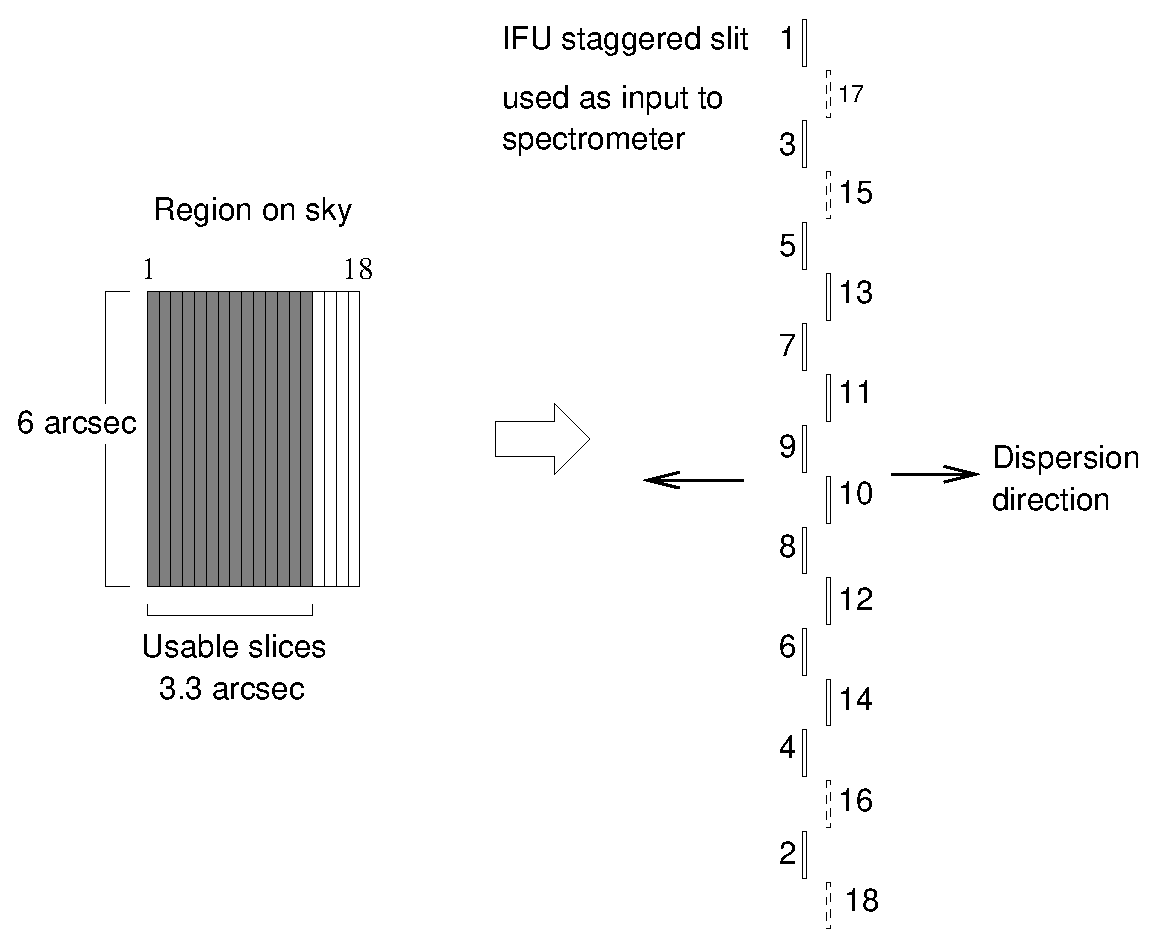
\includegraphics[width=3.5in]{ifu_schematic.eps}
    \caption{A schematic view of the way in which the IFU reformats a
      two dimensional field of view into a staggered column of slices,
      which is then used as the input to the UIST long-slit
      spectrometer (four of the eighteen slices are not usable due to
      misalignment during manufacture of the slicing mirrors).}
    \label{ifu_schematic}
  \end{center}
  \end{figure}
  
  The UIST integral field unit slices a rectangular region of the sky
  into strips and rearranges them in order to use them as the input to
  the UIST long slit spectrometer, as shown in
  Figure~\ref{ifu_schematic}. Note that the slice images on the array
  are not in the same order as the slices on the sky. The offsets from
  one slice to another in the dispersion direction lead to an apparent
  offset in wavelength from one spectrum to another. These data
  reduction recipes are designed to transform this raw output into a
  datacube with ($x$, $y$, $\lambda$) axes, which will be
  divided by a standard-star spectrum and flux calibrated if
  appropriate.


\section{An overview of the reduction}

The first stages of the reduction are common to all types of IFU
observation. In order to reformat the raw output of the IFU into a
datacube it is first necessary to locate the top and bottom of the
spectrum from each slice. The spectra are then extracted and formed
into another 2-d frame in which the spectra are stacked in the order
in which the slices are arranged on the sky. At this stage the spaces
between the spectra are removed and the spectra are shifted in the
dispersion direction in order to align them to approximately the same
wavelength scale (the spectra are shifted by an integer number of
pixels to avoid resampling). These positions and offsets should all
remain constant, so no calibration data needs to be taken for this
stage of the reduction. The data now look very like a conventional
long-slit spectrum. 

The subsequent sequence of the reduction depends on the type of
observation and the recipe used.  If the image is a flat-field frame
then it is now reduced using the conventional spectroscopy flat-field
reduction primitives. If the observation is the first in an object-sky
pair then reduction stops at this point. If it completes a pair then
sky subtraction is now carried out.

The precise alignment of all the spectra is done simultaneously with
wavelength calibration. An arc spectrum is taken and reduced to this
stage. Wavelength calibration of each row in the frame is done using
the \FIGARO\ \xref{{\bf iarc}}{sun86}{IARC} routine. The
wavelength calibrations measured are then applied to subsequent IFU
frames using \xref{{\bf iscrunch}}{sun86}{ISCRUNCH}.

Once we have a frame in which all the rows have been scrunched to the
same wavelength scale we can cut out the 2-d spectrum from each slice
and use each slice as one ($y$, $\lambda$) plane of our ($x$,
$y$, $\lambda$) datacube. Small shifts in $y$ are required to ensure correct
reconstruction of the image (the $x$, $y$ plane), but this is constant
and a predetermined calibration is used.


\section{Flats, Arcs and Standard Stars}

A standard IFU observation sequence consists of a flat and an arc,
followed by observations of the target. The flat is required for
reducing all other IFU observations for flat fielding and for locating
the positions of the slices on the array. The flat is therefore a
mandatory observation for all IFU data reduction. The arc is required
to scrunch all rows of on-sky observations to a common wavelength
scale (note that calibration files for the Krypton lamp are not
available at present - please use only the argon lamp for the
time-being).

It may sometimes be necessary or convenient to postpone observation of
a standard-star until after observing your object. In this case it is
possible to run the {\tt \_NOSTD} versions of the recipes, then re-run the
data reduction once the standard has been observed and reduced.



\section{Displaying reconstructed images}


A `white-light' image will be created from the datacube with the
suffix {\tt \_im} by compressing the datacube over its entire
wavelength range. Other images can be automatically extracted from the
datacube by creating a file in the {\tt \$ORAC\_DATA\_OUT} directory
with the filename {\tt extract.images}. Each line of this file should
contain the desired suffix for the file containing the image (without
the underscore) and either two or four wavelengths (in microns). If a
line contains two wavelengths then an image will be extracted from the
cube between those wavelengths. If four wavelengths are given then two
images will be extracted and the second will be subtracted from the
first. Any lines beginning with {\tt \#} are ignored.

\begin{verbatim}
      # An example extract.images file

      # Extract a broad-band K image
      K   2.1   2.3
      # and a continuum subtracted H_2 1-0 S(1) image
      S1  2.1208   2.1228   2.1250   2.1270
\end{verbatim}

To display these images you will need to edit the {\tt disp.dat} file.
Copy it from the calibration directory to the current reduced data
directory using

\begin{verbatim}
      % cp $ORAC_DATA_CAL/disp.dat $ORAC_DATA_OUT
\end{verbatim}

Images with the suffix {\tt \_im} will be displayed automatically. For
all other images you need to add a line to the {\tt disp.dat} file.
The easiest way of doing this is to use a programme called {\tt
  oracdisp}. Alternatively you can edit the file directly adding a
line which looks like this:

\begin{verbatim}
      S1  tool=kapview type=image window=1 region=1 
\end{verbatim}

See \xref{SUN/230}{sun230}{} for more details on configuring the
\ORACDR\ display system.

Images with the suffix {\tt \_im} will be kept, but all other images
will be deleted at the end of processing as `intermediate files'. If
you include an entry in your {\tt extract.images} file with a suffix
of {im} then this will be extracted and kept instead of the white
light image over the entire wavelength range.

Please note that at present images displayed by \ORACDR\ will be
compressed by a factor of two in the $x$ direction due to the
non-square ($0.24 \times 0.12$ arcsec) pixels of the IFU. The axes
should be correctly labelled with arcsec offsets from the centre of
the field. Images can be displayed with the correct aspect ratio by
running the \KAPPA\ \xref{{\bf display}}{sun95}{DISPLAY} routine with
the options {\tt xmagn=2 ymagn=1} specified on the command line.


\section{Variance propagation}

Poisson and readnoise variances are added to the frame at the start of
the pipeline. These are propagated all the way through the pipeline if
\KAPPA\ 1.0 or newer is used. If an older version of \KAPPA\ is used
then the variance will be lost when the data is formed into a
datacube. A warning will be shown if this happens.

The values of adjacent pixels in the output frame are correlated due
to resampling in the $y$ and $\lambda$ directions, so strictly
speaking the variance of the final frame should be represented by an
enormous covariance array. This would not be practical, so the
variance array is propagated by resampling it in the same way as the
data array, which while not rigorously correct should provide a
useful estimate of the variance.


\section{Data files}

\subsection{Filenames and locations}

At UKIRT, raw data files are stored in {\tt
  /ukirtdata/raw/uist/YYYYMMDD/} (where {\tt YYYYMMDD} is the numeric
UT date).  The files are stored as Starlink HDS containers (files
with multiple data arrays). Each file contains one \emph{observation},
and as such contains a header component and one or more
\emph{integrations}.  Each integration is stored as an NDF component
(single data array) of the HDS file. The raw filenames are {\tt
  uYYYYMMDD\_NNNNN.sdf} where {\tt NNNNN} is the observation number,
padded with leading zeros when necessary.

Reduced data files are written to {\tt
  /ukirtdata/reduced/uist/YYYYMMDD/} or {\tt \$ORAC\_DATA\_OUT}.  The
filename structure is: {\tt (PREFIX)(UTDATE)\_(FRAME
  NUMBER)[\_(SUFFIX)].sdf}.  {\tt PREFIX} is the letter {\tt u} if
the file contains data from a single observation. It is {\tt gu} if
the file contains data from a number of observations (a group).
The suffix is used by individual primitives (think of a primitive as
a single step within a recipe) for their output files. The pipeline
keeps track of passing these files between primitives; useful ones are
left on the disk at the end so you can look at intermediate data
products if you wish (these are marked in the table below).
For example, {\tt u20021031\_00123\_ff.sdf} would be data from a single
observation, number 123, that has been flat fielded (the table below
tells you that {\tt \_ff} means flat fielded). Reduced files can have either
HDS (multiple data arrays) or NDF (single data array) format as
appropriate.

\subsection{File suffixes}

\textbf{Frame suffixes}

\vspace{0.2cm}

\begin{tabular}{l c l}
\hline
Suffix & Kept & Description \hspace{9cm}  \\
\hline
{\tt \_raw} & Y & The raw frame\\
{\tt \_adu} & Y & Scaled to ADUs\\
{\tt \_sbf} & N & Bias frame subtracted\\
{\tt \_pov} & N & Poisson variance added\\
{\tt \_rnv} & N & Readnoise variance added\\
{\tt \_bgl} & N & Shows which pixels are background limited\\
{\tt \_bp}  & N & Bad pixels masked\\
{\tt \_ext} & Y & Slices extracted and approximately aligned\\
{\tt \_ff}  & N & Flat fielded\\
{\tt \_nf}  & Y & Normalised flat\\
{\tt \_bpf} & N & Pixels previously marked as bad filled with
interpolated values\\
{\tt \_ss}  & N & sky-subtracted\\
{\tt \_scr} & Y & All rows scrunched to common wavelength scale\\
{\tt \_cub} & Y & Formed into a datacube\\
{\tt \_dbsc} & N & All spectra in datacube divided by standard\\
{\tt \_im}  & Y & Image extracted from datacube\\
\hline 
\end{tabular}   

\vspace{0.5cm}

\textbf{Group suffixes}

\vspace{0.2cm}

\begin{tabular}{l c l}
\hline
Suffix & Kept & Description \hspace{9cm} \\
\hline
{\tt \_scr} & Y & All rows scrunched to common wavelength scale\\
{\tt \_cub} & Y & Formed into a datacube\\
{\tt \_mos} & Y & Mosaicked datacube\\
{\tt \_dbsc} & Y & All spectra in datacube divided by standard\\
{\tt \_im}  & Y & Image extracted from datacube\\
\hline 
\end{tabular} 


\section{Calibration files}

The calibration files described here are static calibrations which
describe the arrangement of the IFU slice images on the array and the
spectral lines used to wavelength calibrate spectra from each
grism. Standard versions of these files are provided with \ORACDR\ and
you should not need to make any measurements of these calibrations or
make any alterations to these files.

\subsection{The IFU profile}

The lengths and separations of the images of IFU slices are assumed to
be constant. The shifts which are required to align all the spectra in
the dispersion direction ($x$-axis) to an accuracy of $\sim 1$~pixel
and to alpign the slices in the final datacube in the $y$-axis are also
assumed to remain constant. The file {\tt ifu\_profile.dat} in the
{\tt \$ORAC\_DATA\_CAL} directory contains all of these values. 

These values should not change (except after physical adjustments of
the IFU), though refinements in measurement may well be possible.

\subsubsection{File format}

The file contains one line for each slice. Each line contains four
numerical fields separated by white space (any number of spaces or
tabs). The first two give the $y$ positions of the top and bottom of
the slice, the other two give the $x$ and $y$ shift needed to align
the slices. All of these should be integers except for the
$y$-shift. Blank lines and any text following a {\tt \#} will be
ignored. The slices should be listed in the order in which they are
arranged in the two dimensional field of view, not the order in which
they are arranged on the raw IFU image. This is important because the
slices will be put into the final datacube in the order in which they
are listed here.


\subsubsection{Current values}

After commissioning the file {\tt ifu\_profile.dat} contained the
following values.

\begin{verbatim}
      # IFU Profile, measured Jan 2003 using data from 20021205 (SPT)

      # ystart   yend  xshift  yshift 
          743     789      31   -0.10
          286     332      25    0.71
          628     674      26   -0.39
          400     446      24   -0.13
          514     560      22   -0.14
          457     503      -9    4.41
          571     617     -12    2.88
          343     389     -15    4.19
          686     732     -16    4.58
          229     275     -20    4.13
          800     846     -21    5.59
          114     160     -26    3.16
          914     960     -25    4.90
            0      46     -32    3.53
\end{verbatim}


\subsubsection{Measuring the calibration}

The positions of the top and bottom of the slices can be measured in
pixel coordinates from any IFU observation. There is a different
vertical offset for each grism but you do not need to worry about
this because the offset between the positions given and the actual
spectra is measured each time a flat field frame is reduced. 

The $x$-shift values can easily be measured from an arc spectrum.
Values should be chosen to get the arc lines in the {\tt \_ext} file
produced by the {\tt \_EXTRACT\_SLICES\_} primitive as close to being
straight as possible. Integer values should be used because the fine
alignment will happen automatically when all the rows of the spectrum
are scrunched to a common wavelength scale. Inaccurate values will
shift the spectral lines making it difficult for \xref{{\bf
    iarc}}{sun86}{IARC} to wavelength calibrate all the rows.  Using
non-integer values will cause the spectrum to be resampled twice in
the dispersion direction, which is neither necessary or desirable.
Positive values will move the spectrum in the positive $x$ direction.

The $y$-shift value is the most difficult to measure. This shifts each
slice along its length which is necessary for accurate image
reconstruction. This can be measured by using telescope offsets to
scan a star across the field of view of the IFU. The star should be
stepped across the field in steps of approximately one slice width
(0.25 arcsec) then returned to the initial position to check for
systematic drifts. The integrations should be long enough to smooth
the seeing effects.  The datacubes or extracted images can be added
together to produce a horizontal line across the field of view. The
offset from one slice to another can be measured and offsets applied.
A positive value of the $y$-offset will move the slice in the positive
$y$ direction. Note that the plate scale varies slightly from one
slice to another (maximum variation $\sim 3\%$, corresponding to $\sim
1.5$ pixels over the length of the slice) so the offsets should be
measured at the centre of the slices along their length. Alternatively
they can be measured at two positions equal distances from the centre
of the slices in the $y$ direction and the average offset used.





\subsection{Wavelength calibration}
\label{arclines}

Automatic wavelength calibration is significantly easier with a grism
based spectrometer such as UIST than it would be with a grating based
spectrometer such as CGS4. This is because the wavelength calibration of each
grism should be constant to within a pixel or two, whereas the central
wavelength of a grating can be varied continuously over a wide range. 

For each grism there is at least one file in {\tt
  \$ORAC\_DATA\_CAL/grisms/} listing arc lines (there may be more than
one if the grism can sensibly be calibrated with either lamp). These
files have the extension {\tt .lis} and are in the format of the {\tt
  arlines.lis} file produced by the \FIGARO\ \xref{{\bf
    arc}}{sun86}{ARC} task. The appropriate file is found by the
calibration system and copied to {\tt \$ORAC\_DATA\_OUT/arlines.lis}
where it is used by \xref{{\bf iarc}}{sun86}{IARC} to generate a
wavelength calibration for each row of the image.

These arc line lists will need to be re-measured after any change
which will shift the spectra on the array. This includes changes in
the optical alignment of UIST (removing and replacing the grism
wheels, slit wheel, camera wheel or the array). It may also be
necessary to generate new calibrations if the $x$-shift values in {\tt
  ifu\_profile.dat} are changed significantly.


\subsubsection{File format}

You are unlikely to need to worry about the format of the arc lines
files. These files are produced by \xref{{\bf arc}}{sun86}{ARC} and
used by \xref{{\bf iarc}}{sun86}{IARC}. For details of the format
please see the \FIGARO\ documentation.

A typical file looks like this (the arc lines for the short-$J$ grism
with the argon lamp):

\begin{verbatim}
      4 lines identified from /home/spt/oracdr_cal/uist/grisms/arcs/short_J_Ar

        Channel   Wavelength   Calculated  Discrepancy  Line#
        67.1694   11671.9004   11671.9150       0.0146      1    
       185.4290   11491.2002   11491.1787      -0.0215      2    
       727.9574   10676.5000   10676.5186       0.0186      3    
       866.0963   10472.9004   10472.8877      -0.0127      4    

      RMS error:       0.02, Line width used:  2.00

      Order of fit:   2

      0.4040299644214860E-04-0.1538503512984496E+01 0.1177507315490152E+05
\end{verbatim}

The only part of this file to be directly used by any of the recipes
(rather than by a \FIGARO\ task) is the final line, giving the
polynomial wavelength fit, which is used to calculate the wavelength
range to which the spectra should be scrunched.

\subsubsection{Measuring the calibration}

To generate a new arc lines list file you will first need to reduce a
flat-field frame as normal, then reduce an arc using the {\tt
  EXTRACT\_SLICES} recipe. This will extract the slices from the
array, approximately align them in wavelength and apply the
flat-field. The frame is now in the state that arc frames will be in
when they are wavelength calibrated. 

Extract a spectrum from the central slice, (or the one before if there
are an even number of slices), so for UIST extract a spectrum from the
7th slice from the bottom. This is where \xref{{\bf
    iarc}}{sun86}{IARC} starts its fitting. Copy the spectrum to {\tt
  \$ORAC\_DATA\_CAL/grisms/arcs/} and give it a meaningful name (e.g.\ 
{\tt short\_K\_Ar.sdf}). This is not essential because the spectrum is
not used for calibration but it will include all the headers
describing the instrument configuration at the time, which may be
useful for future reference.

Use \FIGARO\ \xref{{\bf arc}}{sun86}{ARC} to wavelength calibrate the
spectrum. The wavelength calibration should be in Angstroms. A 2nd or
3rd order fit is likely to be most appropriate. \xref{{\bf
    arc}}{sun86}{ARC} will generate a file called {\tt arlines.lis}.
This is the arc lines file that you want. Give it a more useful name
(e.g.\ {\tt short\_K\_Ar.lis}) and put it in {\tt
  \$ORAC\_DATA\_CAL/grisms/}.

In order for the calibration system to know about the file you will
need to add it to the {\tt index.arlines} file which you will find in
the {\tt \$ORAC\_DATA\_CAL/} directory.

\section{Index files}

When calibration files are reduced they are listed in an index file in
the directory containing the reduced data. Where separate index files
are used by imaging and spectroscopy recipes (e.g.\ {\tt
  index.flat\_im and index.flat\_sp}) the spectroscopy files will be
used. Two of the index files used include more information than just
the filename of the calibration frames.

The {\tt index.iar} file indexes not only the {\tt .iar} files
generated by \FIGARO\ \xref{{\bf iarc}}{sun86}{IARC} containing the
wavelength calibration of every row but also the wavelength range (in
Angstroms) to which the spectra should be scrunched. The filename and
the minimum and maximum wavelengths are separated by colons.

\begin{verbatim}
      #GRISM ORACTIME
      u20030131_00011_bpf.iar:14081:24988 HK+ifu 4.911111
      u20030131_00067_bpf.iar:20159:22489 short_K+ifu 7.316945
\end{verbatim}

Similarly, the {\tt index.offset} file contains both the name of the
file from which the offset value was measured and the offset itself
separated by a colon.

\begin{verbatim}
      #GRISM ORACTIME
      u20030131_00010.I1:26 HK+ifu 4.905833
      u20030131_00066.I1:19 short_K+ifu 7.297500
\end{verbatim}

There is also one index file, {\tt index.arlines}, which is not stored
in the reduced data directory but in the calibration directory ({\tt
  \$ORAC\_DATA\_CAL}). This is the index of the arc lines lists (see
section \ref{arclines}), which are static calibration files.

\section{IFU headers}

The {\tt ifu\_profile.dat} and the appropriate grism data file are read
by the {\tt \_LOCATE\_SLICES\_} primitive, which does nothing to the
frame except put the positions of the slices and the offsets which
should be applied to them into the header of the frame for use by
subsequent primitives. The values are written into the entries {\tt
  IFU\_start}, {\tt IFU\_end}, {\tt IFU\_xshift} and {\tt
  IFU\_yshift}. Each of these headers contains an $n$ element array
(indices 0 to $n-1$), where $n$ is the number of slices. An additional
header entry, {\tt IFU\_slices}~$=n$, is also written.

When the positions of the slices in the frame is changed by a
primitive (for example, when the slices are re-ordered and shifted by
the {\tt \_EXTRACT\_SLICES\_} primitive) the new positions of the
slices should be written into the header of the output file to be
available for subsequent primitives.




\clearpage

%\appendix

\section{Recipes}

\subsection{EXTENDED\_SOURCE}

Produce a coadded, sky-subtracted, wavelength-calibrated,
flux-calibrated datacube from a group of SKY-OBJECT pairs of IFU
frames.

\subsubsection*{Description\index{Description}}

Read-noise and Poisson variances are added to the frame and a bad
pixel mask is applied. The spectrum from each slice of the IFU is cut
out of the frame and pasted in a new frame in such a way that there
are no longer spaces between the spectra, the spectra are arranged in
the order in which they appear in the field of view and they are
approximately aligned in the dispersion direction. The spectrum is
flat-fielded and sky-object pairs are now subtracted.  The wavelength
calibration previously measured from the arc spectrum is used to apply
a common, linear wavelength scale to each row of the the
sky-subtracted 2-d spectrum.  The resulting frame is coadded to the
group, which is then rearranged to form a data-cube. The spectral
dimension of the data-cube is divided by the standard-star spectrum
and flux calibrated. Images can be extracted over a range of
wavelengths specified in a file called {\tt extract.images} placed in
the {\tt \$ORAC\_DATA\_OUT} directory, and can be displayed by editing
the {\tt disp.dat} file.

\subsubsection*{Notes\index{Notes}}\begin{itemize}
\item 

A suitable flat-field spectrum, arc spectrum and standard-star
spectrum should previously have been reduced and filed with the
calibration system.

\item 

  Sky-object pairs may be observed in any sequence (for example
  sky-object-object-sky or object-sky-object-sky). Any observations
  with telescope offsets greater than 30 arcsec will be assumed to be
  a sky position. It is recommended that the observation types are set
  to OBJECT and SKY as appropriate (this is essential if your offsets
  to sky are smaller than 30 arcsec).

\item

Variances are propagated if \KAPPA\ 1.0 or later is available. A warning
is displayed if variances are lost.

\item 

A variant of this recipe, EXTENDED\_SOURCE\_NOSTD, is
available which does not divide the spectrum by a standard-star or
flux calibrate the spectrum. It may be useful to specify this recipe
on the command line when running \ORACDR\ if you choose to defer
observation of your standard until after you have observed your
object.

\end{itemize}

\subsubsection*{Output data}

The individual frames with slices extracted and approximately aligned
have the suffix {\tt \_ext}. The flat-fielded, scrunched,
sky-subtracted pairs have the suffix {\tt \_scr}. 

Several group files are created (with names starting {\tt gu\_}). The
coadded scrunched 2-d spectrum has the suffix {\tt \_scr}. This is
formed into a datacube with the suffix {\tt \_cub}. A cube which has
been divided by the standard-star spectrum is formmed with the suffix
{\tt \_dbsc} and a flux calibrated datacube with the suffix {\tt
  \_fc}.  A white-light image is extracted from this datacube with the
suffix {\tt \_im}.

\clearpage


\subsection{EXTENDED\_SOURCE\_NOSTD}

Produce a coadded, sky-subtracted, wavelength-calibrated,
datacube from a group of SKY-OBJECT pairs of IFU
frames.

\subsubsection*{Description\index{Description}}

Read-noise and Poisson variances are added to the frame and a bad
pixel mask is applied. The spectrum from each slice of the IFU is cut
out of the frame and pasted in a new frame in such a way that there
are no longer spaces between the spectra, the spectra are arranged in
the order in which they appear in the field of view and they are
approximately aligned in the dispersion direction. The spectrum is
flat-fielded and sky-object pairs are now subtracted.  The wavelength
calibration previously measured from the arc spectrum is used to apply
a common, linear wavelength scale to each row of the the
sky-subtracted 2-d spectrum.  The resulting frame is coadded to the
group, which is then rearranged to form a data-cube. The spectral
dimension of the data-cube is divided by the standard-star spectrum
and flux calibrated. Images can be extracted over a range of
wavelengths specified in a file called {\tt extract.images} placed in
the {\tt \$ORAC\_DATA\_OUT} directory, and can be displayed by editing
the {\tt disp.dat} file.

\subsubsection*{Notes\index{Notes}}\begin{itemize}
\item 
  
  A suitable flat-field spectrum and arc spectrum should previously
  have been reduced and filed with the calibration system.

\item 

  Sky-object pairs may be observed in any sequence (for example
  sky-object-object-sky or object-sky-object-sky). Any observations
  with telescope offsets greater than 30 arcsec will be assumed to be
  a sky position. It is recommended that the observation types are set
  to OBJECT and SKY as appropriate (this is essential if your offsets
  to sky are smaller than 30 arcsec).

\item

Variances are propagated if \KAPPA\ 1.0 or later is available. A warning
is displayed if variances are lost.


\item 
  
  This is a variant of EXTENDED\_SOURCE which does not divide the
  spectrum by a standard-star or flux calibrate the spectrum. This
  recipe should be specified on the command line when running
  \ORACDR\ if you choose to defer observation of your standard until
  after you have observed your object.

\end{itemize}

\subsubsection*{Output data}

The individual frames with slices extracted and approximately aligned
have the suffix {\tt \_ext}. The flat-fielded, scrunched,
sky-subtracted pairs have the suffix {\tt \_scr}. No datacube is
formed from individual frames or pairs.

Several group files are created (with names starting {\tt gu\_}). The
coadded scrunched 2-d spectrum has the suffix {\tt \_scr}. This is
formed into a datacube with the suffix {\tt \_cub}. A white-light image is
extracted from this datacube with the suffix {\tt \_im}.


\clearpage
\subsection{MAKE\_CAL\_ARC}



Reduces an IFU arc frame to the stage that it can be used to generate
an arc-lines list.

\subsubsection*{Description\index{Description}}

This recipe reduces a single IFU arc frame to a form that can be used
to generate an arc lines list file. These are static calibration files
stored in {\tt \$ORAC\_DATA\_CAL/grisms/}, which should rarely need to
be re-generated.  


Read-noise and Poisson variances are added to the frame and a bad
pixel mask is applied. The spectrum from each slice of the IFU is cut
out of the frame and pasted in a new frame in such a way that there
are no longer spaces between the spectra, the spectra are arranged in
the order in which they appear in the field of view and they are
approximately aligned in the dispersion direction. The spectrum is
flat-fielded.


\subsubsection*{Notes\index{Notes}}

\begin{itemize}
\item 
  
  A suitable flat-field spectrum should previously
  have been reduced and filed with the calibration system.

\item 

Variances are propagated.

\item

Observers should not need this recipe.

\end{itemize}

\clearpage

\subsection{MAP\_EXTENDED\_SOURCE}

Reduce a group of sky-object pairs of IFU frames, mosaicking datacubes
using telescope offsets.

\subsubsection*{Description\index{Description}}

This recipe produces a coadded, sky-subtracted, wavelength-calibrated,
flux-calibrated datacube from a group of sky-object pairs of IFU
frames. The telescope offsets are used to mosaic datacubes together,
allowing a region larger than the field of view of the IFU to be
mapped.



Read-noise and Poisson variances are added to the frame and a bad
pixel mask is applied. The spectrum from each slice of the IFU is cut
out of the frame and pasted in a new frame in such a way that there
are no longer spaces between the spectra, the spectra are arranged in
the order in which they appear in the field of view and they are
approximately aligned in the dispersion direction. The spectrum is
flat-fielded and the wavelength calibration measured from the arc
spectrum is used to apply a common, linear wavelength scale to each
row of the 2-d spectrum.



Sky-object pairs are now subtracted, and the resulting frame is
rearranged to form a data-cube, which is divided by the standard-star
spectrum, flux calibrated and mosaicked into the group.


\subsubsection*{Notes\index{Notes}}\begin{itemize}
\item 
  
  A suitable flat-field spectrum, arc spectrum and standard-star
  spectrum should previously have been reduced and filed with the
  calibration system.

\item 

It is recommended that the observation types of the observations are set
to OBJECT and SKY as appropriate. This is inconvenient if you wish to
set up a sequence using an offset iterator in \textsc{orac-ot}, so any frames
with a telescope offset greater than 30~arcsec will be assumed to be a
sky position.

\item 

Variances are propagated if \KAPPA\ 1.0 or later is available. A warning
is displayed if variances are lost.

\item 

Any number of sky-object pairs in any jitter pattern may be used.

\item
A variant of this recipe, {\tt MAP\_EXTENDED\_SOURCE\_NOSTD}, is
available which does not divide the spectrum by a standard-star or
flux calibrate the spectrum. It may be useful to specify this recipe
on the command line when running \ORACDR\ if you choose to defer
observation of your standard until after you have observed your
object.

\end{itemize}

\subsubsection*{Output data}

The individual frames with slices extracted and approximately aligned
have the suffix {\tt \_ext}. The flat-fielded, scrunched,
sky-subtracted pairs have the suffix {\tt \_scr}. A datacube is
formed from each pair with the suffix {\tt \_cub}.

The datacubes are mosiaced into a file with the suffix {\tt \_mos}. A
white-light image is extracted from this datacube with the suffix {\tt
  \_im}.

\clearpage

\subsection{MAP\_EXTENDED\_SOURCE\_NOSTD}

Reduce a group of sky-object pairs of IFU frames, mosaicking datacubes
using telescope offsets.

\subsubsection*{Description\index{Description}}

This recipe produces a coadded, sky-subtracted, wavelength-calibrated,
datacube from a group of sky-object pairs of IFU
frames. The telescope offsets are used to mosaic datacubes together,
allowing a region larger than the field of view of the IFU to be
mapped.



Read-noise and Poisson variances are added to the frame and a bad
pixel mask is applied. The spectrum from each slice of the IFU is cut
out of the frame and pasted in a new frame in such a way that there
are no longer spaces between the spectra, the spectra are arranged in
the order in which they appear in the field of view and they are
approximately aligned in the dispersion direction. The spectrum is
flat-fielded and the wavelength calibration measured from the arc
spectrum is used to apply a common, linear wavelength scale to each
row of the 2-d spectrum.



Sky-object pairs are now subtracted, and the resulting frame is
rearranged to form a data-cube, which is mosaicked into the group.


\subsubsection*{Notes\index{Notes}}\begin{itemize}
\item 
  
  A suitable flat-field spectrum and arc spectrum should previously
  have been reduced and filed with the calibration system.

\item 

It is recommended that the observation types of the observations are set
to OBJECT and SKY as appropriate. This is inconvenient if you wish to
set up a sequence using an offset iterator in \textsc{orac-ot}, so any frames
with a telescope offset greater than 30~arcsec will be assumed to be a
sky position.

\item 

Variances are propagated if \KAPPA\ 1.0 or later is available. A warning
is displayed if variances are lost.

\item 

Any number of sky-object pairs in any jitter pattern may be used.

\item 
    This is a variant of MAP\_EXTENDED\_SOURCE which does not divide the
  spectrum by a standard-star or flux calibrate the spectrum. This
  recipe should be specified on the command line when running
  \ORACDR\ if you choose to defer observation of your standard until
  after you have observed your object.
  

\end{itemize}

\subsubsection*{Output data}

The individual frames with slices extracted and approximately aligned
have the suffix {\tt \_ext}. The flat-fielded, scrunched,
sky-subtracted pairs have the suffix {\tt \_scr}. A datacube is
formed from each pair with the suffix {\tt \_cub}.

The datacubes are mosiacked into a file with the suffix {\tt \_mos}. A
white-light image is extracted from this datacube with the suffix {\tt
  \_im}.

\clearpage

\subsection{NIGHT\_LOG}

Creates a text log summarising file headers

\subsubsection*{Description}

This recipe is used to create a text log summarising the file headers
of a group of observations. It is often used to create a log file
describing a whole night's worth of observations.

For full details, see the documentation for the spectroscopy
\_NIGHT\_LOG\_ primitive.



This recipe calls the primitive in such a way that the log file
appears in {\tt \$ORAC\_DATA\_IN}.

An `on-the-fly' night log is created in {\tt \$ORAC\_DATA\_OUT} as 
spectroscopy data is reduced by the pipeline. This is done by a
call to \_NIGHT\_LOG\_ from \_SPECTROSCOPY\_HELLO\_.

\subsubsection*{See also}

The spectroscopy recipe: NIGHT\_LOG\\
The ifu recipe: NIGHT\_LOG\_LONG\\
The ifu primitive: \_NIGHT\_LOG\_


\subsection{NIGHT\_LOG\_LONG}

Creates a text log detailing file headers

\subsubsection*{Description}

This recipe does the same as the NIGHT\_LOG recipe, except that it
produces a more detailed log.

\subsubsection*{See also}

The spectroscopy recipe: NIGHT\_LOG\_LONG\\
The ifu recipe: NIGHT\_LOG\\
The ifu primitive: \_NIGHT\_LOG\_



\clearpage

\subsection{REDUCE\_ARC}



Reduces an IFU arc spectrum

\subsubsection*{Description\index{Description}}

This recipe is used to reduce an IFU arc spectrum. A wavelength
calibration is obtained for each row of the spectrum. The file
containing these calibrations is filed with the calibration system and
used to apply a common, linear wavelength calibration to all rows of
subsequent observations.



Read-noise and Poisson variances are added to the frame and a bad
pixel mask is applied. The spectrum from each slice of the IFU is cut
out of the frame and pasted in a new frame in such a way that there
are no longer spaces between the spectra. The spectra are now arranged
in the order in which they appear in the field of view and
approximately aligned in the dispersion direction. The spectrum is
divided by the flat-field.



The Figaro Iarc task is then used to obtain a wavelength calibration for
each row, using a pre-calibrated arc file to provide the initial
fit. Finally all the rows are scrunched to a common, linear wavelength
scale to allow the observer to check that the wavelength calibration
was correct (i.e. that the spectra are now straight). 

\subsubsection*{Notes\index{Notes}}\begin{itemize} 

\item 

A flat-field spectrum must have been reduced and filed as a calibration.
This is essential for locating the positions of the spectra.

\item

The spectrum from each slice is smoothed with a $1 \times 6$-pixel box
filter before wavelength calibration, primarily to cover bad pixels.

\item 

Variances are propagated, but are not used by Iarc when wavelength
calibrating. 

\item

The arc is wavelength calibrated using a list of arc lines from a
pre-calibrated arc spectrum to provide an initial fit. These are
expected to be constant and are stored in the {\tt \$ORAC\_DATA\_CAL/grisms/}
directory. The appropriate file (same grism and arc lamp) is provided 
by the calibration system.

\item 

The recipe checks the r.m.s.\ value of the wavelength fit returned by
Iarc, and will warn the user if this value seems too high. The
observer is recommended to always look at the scrunched arc frame. If
the wavelength calibration has worked successfully then all the arc
lines should be straight, and the frame should be virtually
indistinguishable from a long-slit spectrum.


\end{itemize}

\subsubsection*{Output data}

A file giving the wavelength calibration to be applied to each row is
generated with a filename extension of {\tt .iar}. 

A file containing the arc frame with all rows scrunched to a common
wavelength scale is produced with a suffix of {\tt \_scr}.

\clearpage


\subsection{REDUCE\_FLAT}

Reduces an IFU flat field

\subsubsection*{Description\index{Description}}

This recipe is used to reduce an IFU flat-field spectrum. The
normalised flat is filed with the calibration system.

The relative positions of the slice spectra on the array are contained
in a static look-up table. The flat field frame is used to measure the
offset of these positions (they are shifted vertically by different
amounts for different grisms). This value is filed with the calibration
system for use when reducing subsequent frames.

The separate slice spectra are extracted from the frame and rearranged
in a new 2-d frame in the correct order (the order in which they cover
the 2-d field of view) and approximately aligned in the spectral axis. This 
produces a frame that looks more like a long-slit spectrum.

The frame is now treated as a standard long-slit spectrum. The image
is collapsed in the $y$-direction, a black-body spectrum is fitted to
this and all rows of the flat field are divided by this spectrum to
remove the characteristics of the lamp from the flat-field (this does
not have to be done precisely because the same flat-field is used for
object frames and flux calibrators, so it cancels out anyway). The
image is normalised to have a mean value of 1.  The flat field is
filed with the calibration system.




\subsubsection*{Notes\index{Notes}}
\begin{itemize}

\item

Variances are propagated.

\item

The flat-field accounts for the difference in transmission from one
slice to another as well as pixel to pixel variation.

\item
  
  The flat field is used to find the offset between the $y$-positions
  of the spectra from each slice and the positions given in {\tt
    \$ORAC\_DATA\_CAL/ifu\_profile.dat}. The offset measured is stored
  in {\tt index.offset}.

\end{itemize}

\subsubsection*{Output data}

The normalised flat is stored in {\tt flat\_<n>}, where {\tt <n>} is
the observation number.

\clearpage

\subsection{REDUCE\_SINGLE\_FRAME}



Reduces a single IFU frame, producing a wavelength calibrated datacube

\subsubsection*{Description\index{Description}}

This recipe reduces a single IFU frame (i.e. no sky subtraction or
coadding is carried out).



Read-noise and Poisson variances are added to the frame and a bad
pixel mask is applied. The spectrum from each slice of the IFU is cut
out of the frame and pasted in a new frame in such a way that there
are no longer spaces between the spectra, the spectra are arranged in
the order in which they appear in the field of view and they are
approximately aligned in the dispersion direction. The spectrum is
flat-fielded and the wavelength calibration measured from the arc
spectrum is used to apply a common, linear wavelength scale to each
row of the the 2-d spectrum.



Once all the rows of the image are scrunched to a common linear wavelength 
scale the 2-d spectrum from each slice is cut out and used to form
a single ($y$, $\lambda$) plane of the ($x$, $y$, $\lambda$) datacube.

\subsubsection*{Notes\index{Notes}}

\begin{itemize}
\item 
  
  A suitable flat-field spectrum and arc spectrum should previously
  have been reduced and filed with the calibration system.

\item 

Variances are propagated if \KAPPA\ 1.0 or later is available. A warning
is displayed if variances are lost.
\end{itemize}

\clearpage



\subsection{STANDARD\_STAR}

Reduce IFU standard-star observations with a separate sky position

\subsubsection*{Description\index{Description}}

Take a series of standard-star observations and extract and file a
standard-star spectrum. This recipe is designed for use when an offset
sky position has been used. The frames are subtracted in pairs, giving
a sky-subtracted spectrum, which is extracted using optimal
extraction. The spectral type and magnitude of the star is obtained
from the Simbad database. The resulting spectrum is divided by a
black-body spectrum of the appropriate temperature and filed as a
calibration frame.

\subsubsection*{Notes\index{Notes}}\begin{itemize}

\item 
  
  A suitable flat-field spectrum and arc spectrum should previously
  have been reduced and filed with the calibration system.

\item
  
  Sky-object pairs may be observed in any sequence (for example
  sky-object-object-sky or object-sky-object-sky). Any observations
  with telescope offsets greater than 30 arcsec will be assumed to be
  a sky position. It is recommended that the observation types are set
  to OBJECT and SKY as appropriate (this is essential if your offsets
  to sky are smaller than 30 arcsec).

\item

  Variances are propagated.

\item 
  
  Based on the spectroscopy recipe of the same name, and uses
  spectroscopy primitives.

\item 

A datacube is formed of each subtracted pair and an image is extracted
to allow you to confirm that your target is suitably located on the
field, but no coadded datacube is formed.

\end{itemize}

\subsubsection*{See also}

STANDARD\_STAR\_NOD\_ON\_IFU

\subsubsection*{Output data}

The standard-star spectrum divided by a black-body spectrum will be written to
a file with the name {\tt std\_<n>\_sp}. A datacube in which every
$(x,y)$ position contains this spectrum is created with the name {\tt
  std\_<n>\_cube}.

\clearpage



\subsection{STANDARD\_STAR\_NOD\_ON\_IFU}

Reduce IFU standard-star observations when the star
has been offset within the field of the IFU.

\subsubsection*{Description\index{Description}}

Take a series of standard-star observations and extract and file a
standard-star spectrum. This recipe is designed for use when the star
has been offset within the field of the IFU (similar to offsetting
along the slit in conventional spectroscopy). The frames are
subtracted in pairs, giving a positive and negative spectrum. The two
spectra are extracted using optimal extraction and averaged. The
resulting spectrum is divided by a black-body spectrum of the
appropriate temperature and filed as a calibration frame.

\subsubsection*{Notes\index{Notes}}\begin{itemize}
\item 

A suitable flat-field spectrum and arc spectrum should previously have
been reduced and filed with the calibration system.

\item

  Variances are propagated.

\item 

A datacube is formed of each subtracted pair and an image is extracted
to allow you to confirm that your target is suitably located on the
field, but no coadded datacube is formed.

\end{itemize}

\subsubsection*{See also}

STANDARD\_STAR

\subsubsection*{Output data}

The standard-star spectrum divided by a black-body spectrum will be
written to a file with the name {\tt std\_<n>\_sp}. A datacube in
which every $(x,y)$ position contains this spectrum is created with
the name {\tt std\_<n>\_cube}.

\clearpage










\end{document}